\subsection{Package description}

The \textit{trajectory\_tracker} package is responsible for two main tasks:
\begin{itemize}
	\item generating the setpoints of the desired trajectory;
	\item applying the control law to make the robot track such trajectory.
\end{itemize} 

\begin{figure}[H]
\makebox[\textwidth][c]{
\begin{tikzpicture}%[scale=0.6, every node/.style={scale=0.6}]
	\node[
		draw,
		fill=BlueGreen,
		minimum height=1.5cm
	] (generator) {\begin{tabular}{c} Trajectory \\ Generator \end{tabular}};
	
	\node[
		draw,
		fill=BlueGreen,
		minimum height=1.5cm,
		right= of generator,
	] (refTransform) {\begin{tabular}{c} Reference \\ Transformation \end{tabular}};
	
	\node[
		draw,
		fill=BlueGreen,
		minimum height=5cm,
		right = of refTransform,
		shift = {(0cm,-1.75cm)}
	] (trackingLaw) {\begin{tabular}{c} Trajectory \\ Tracker \end{tabular}};
	
	\node[
		draw,
		fill=BlueGreen,
		minimum height=1.5cm,
		below = 2 of refTransform
	] (outputTransform) {\begin{tabular}{c} Output \\ Transformation \end{tabular}};

	\node[
		draw,
		fill=Apricot,
		minimum height=1.5cm,
		below = 2 of generator
	] (odom) {\begin{tabular}{c} $/vesc/odom$ \end{tabular}};

	\node[
		draw,
		fill=Lavender,
		minimum height=1.5cm,
		right = of trackingLaw
	] (controlPackage) {\begin{tabular}{c} $car\_kinematic\_linearizer$ \end{tabular}};

	% trajectory generator node incoming arrows
	\draw[-{Triangle}]  ($(generator.north) + (-0.5, 1)$) -- ($(generator.north) + (-0.5, 0)$)
		node[above, pos=0.2]{\scriptsize \begin{tabular}{c} Desired \\ Trajectory \\ Shape \end{tabular}};

		\draw[-{Triangle}]  ($(generator.north) + (0.5, 1)$) -- ($(generator.north) + (0.5, 0)$)
		node[above, pos=0.10]{$t$};
	
	% reference transformation node incoming arrows
	\draw[-{Triangle}] ($(odom.east) + (0, +1/2)$) -- ++(0.55cm,0) |- ($(refTransform.south) - (0,1)$)  -- ($(refTransform.south)$);

	\draw[-{Triangle}] ($(generator.east) + (0, +1/3)$) -- ($(refTransform.west) + (0, +1/3)$)
		node[midway, above]{$x_{ref}$};
		
	\draw[-{Triangle}] ($(generator.east) + (0, -1/3)$) -- ($(refTransform.west) + (0, -1/3)$)
		node[midway, above]{$y_{ref}$};

	% trajectory tracking law node incoming arrows
	\draw[-{Triangle}] ($(refTransform.east) + (0, +1/3)$) -- ($(trackingLaw.west) + (0,1.75+1/3)$)
		node[midway, above]{$x_{P_{ref}}$};
		
	\draw[-{Triangle}] ($(refTransform.east) + (0, -1/3)$) -- ($(trackingLaw.west) + (0,1.75-1/3)$)
		node[midway, above]{$y_{P_{ref}}$};

	\draw[-{Triangle}] ($(outputTransform.east) + (0, +1/3)$) -- ($(trackingLaw.west) + (0,-1.75+1/3)$)
		node[midway, above]{$x_{P}$};
		
	\draw[-{Triangle}] ($(outputTransform.east) + (0, -1/3)$) -- ($(trackingLaw.west) + (0,-1.75-1/3)$)
		node[midway, above]{$y_{P}$};

	% output transformation node incoming arrows
	
	\draw[-{Triangle}] ($(odom.east) + (0, +1/2)$) -- ($(outputTransform.west) + (0,+1/2)$)
		node[midway, above]{$\theta$};
		
	\draw[-{Triangle}] ($(odom.east)$) -- ($(outputTransform.west)$)
		node[midway, above]{$x$};

	\draw[-{Triangle}] ($(odom.east) + (0, -1/2)$) -- ($(outputTransform.west) + (0,-1/2)$)
		node[midway, above]{$y$};

	% controlPackage node incoming arrows
	\draw[-{Triangle}] ($(trackingLaw.east) + (0, +1/3)$) -- ($(controlPackage.west) + (0,+1/3)$)
		node[midway, above]{$v_{x_{_{P}}}$};
		
	\draw[-{Triangle}] ($(trackingLaw.east) + (0, -1/3)$) -- ($(controlPackage.west) + (0,-1/3)$)
		node[midway, above]{$v_{y_{_{P}}}$};

	% legend
	\matrix [draw,below left] at (current bounding box.north east) {
 	\node [draw, fill= BlueGreen,label=right:\tiny trajectory\_tracker node] () {}; \\
	\node [draw, fill= Apricot,label=right:\tiny ROS topic] () {}; \\
	\node [draw, fill= Lavender,label=right:\tiny other package] () {}; \\
	};

\end{tikzpicture}}
\caption{trajectory\_tracker package schematic}
\end{figure}

The main components of the package are:
\begin{itemize}
	\item[\textcolor{BlueGreen}{$\blacksquare$}] \textbf{Trajectory Generator} which is in charge of computing the appropriate 
		setpoint given the desired trajectory shape and the time $t$ elapsed since the starting of the motion. \\
		The implemented trajectory shapes are:
		\begin{itemize}
			\item[$\blacktriangleright$] Line, a simple linear path described by equations:
				\[ x_{ref} = at \qquad (\dot{x_{ref}} = a) \]
				\[ y_{ref} = bt \qquad (\dot{y_{ref}} = b) \] 
				Where $a$ and $b$ determine the direction (the line is parallel to the direction vector $\vec{d}=(a,b)$) and the speed of the trajectory;
				
				\begin{figure}[H]
				\makebox[\textwidth][c]{
					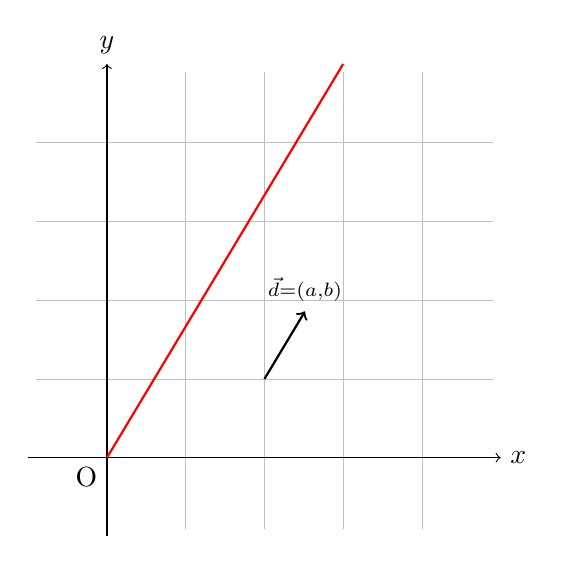
\begin{tikzpicture}
						\draw[gray,very thin, opacity = 0.5] (-0.9,-0.9) grid (4.9,4.9) [step=0.25cm];
						\draw[->] (-1,0) -- (5,0) node[right] {$x$};
						\draw[->] (0,-1) -- (0,5) node[above] {$y$};
						\draw[] (0,0) node[below left] {O};

						\draw[-, color=Red, thick] (0,0) -- (3,5) node[above] {};
						\draw[->, thick] (2,1) -- (2.5145,1.857) node[above] {$\scriptstyle \vec{d}=(a,b)$};
					\end{tikzpicture}}
				\caption{Linear trajectory (where $\vec{d}=(3,5)$)}
				\end{figure}	

			\item[$\blacktriangleright$] Parabola, a parabolic path described by equations: 
				\[x_{ref} = 2at \qquad (\dot{x_{ref}} = 2a)\]
				\[y_{ref} = at^2 \qquad (\dot{y_{ref}} = 2at)\]
				Where $a$ is the focal length of the parabola;
				
				\begin{figure}[H]
				\makebox[\textwidth][c]{
					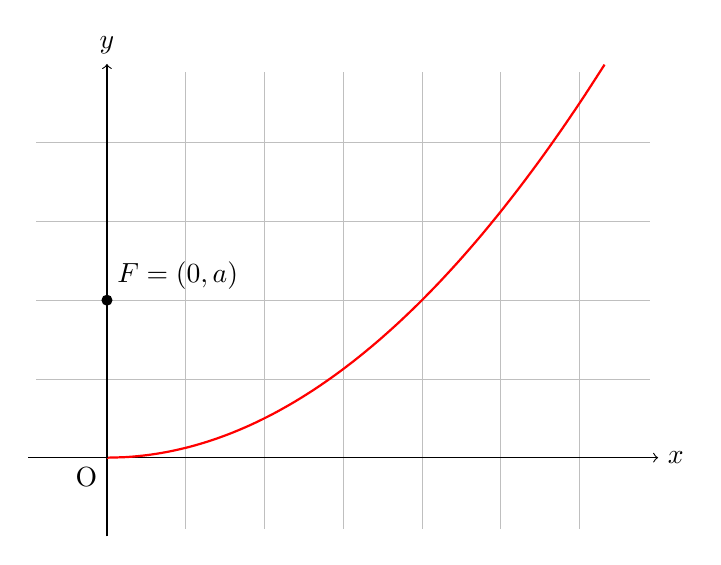
\begin{tikzpicture}
						\draw[gray,very thin, opacity = 0.5] (-0.9,-0.9) grid (6.9,4.9) [step=0.25cm];
						\draw[->] (-1,0) -- (7,0) node[right] {$x$};
						\draw[->] (0,-1) -- (0,5) node[above] {$y$};
						\draw[] (0,0) node[below left] {O};

						% draw parabola having a = 2
						\draw[thick, color = red ,variable=\t,domain=0.0:1.58, smooth]
							plot ({\t*2*2},{2*\t^2});
						\draw[-, thick] (0,0) -- (0,2) node[above right] {$F=(0,a)$};
						\fill (0,2)    circle (2pt);
					\end{tikzpicture}}
				\caption{Parabolic trajectory (where $a = 2$)}
				\end{figure}

			\item[$\blacktriangleright$] Circle, a circular path described by equations:
				\[x_{ref} = r\cos(\omega t - \frac{\pi}{2}) \qquad (\dot{x_{ref}} = -\omega r\sin(\omega t - \frac{\pi}{2})) \]
				\[y_{ref} = r\sin(\omega t - \frac{\pi}{2}) + r \qquad (\dot{y_{ref}} = \omega r\cos(\omega t - \frac{\pi}{2})) \]
				Where $r$ is the radius of the circumference and $\omega$ is the angular velocity. \\
				Since the robot starts at (0,0), a phase shift of $\frac{\pi}{2}$ and an offset of $r$ on the
				y axis are needed so to have a continuos trajectory (to have it starting at (0,0) when $t=0$).

				\begin{figure}[H]
					\makebox[\textwidth][c]{
						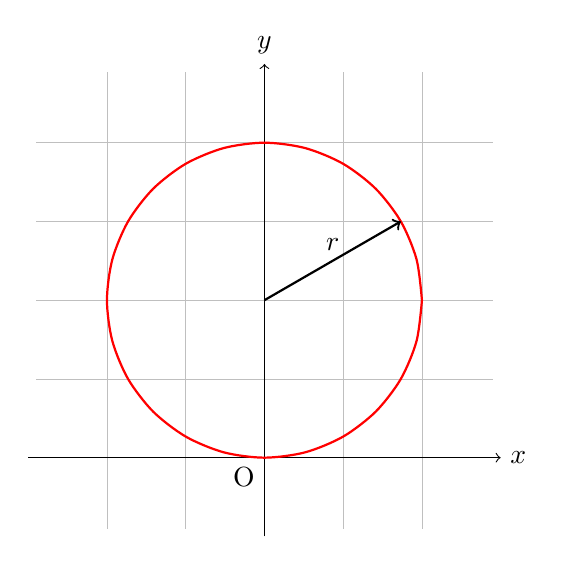
\begin{tikzpicture}
							\draw[gray,very thin, opacity = 0.5] (-2.9,-0.9) grid (2.9,4.9) [step=0.25cm];
							\draw[->] (-3,0) -- (3,0) node[right] {$x$};
							\draw[->] (0,-1) -- (0,5) node[above] {$y$};
							\draw[] (0,0) node[below left] {O};
	
							% draw circle having r = 2
							\draw[thick, color = red ,variable=\t,domain=0.0:360, smooth]
								plot ({2 * cos(\t)},{2 * sin(\t) + 2});
							\draw[->, thick] (0,2) -- node[above] {$r$} ++ ({2 * cos(30)},{2 * sin(30)}) ;
						\end{tikzpicture}}
					\caption{Circular trajectory (where $r = 2$)}
					\end{figure}
	
			\item[$\blacktriangleright$] Figure Eight, an eight shaped path described by equations:
				\[x_{ref} = a\sin(\omega t) \qquad (\dot{x_{ref}} = wa\cos(\omega t)) \]
				\[y_{ref} = a\sin(\omega t)\cos(\omega t) \qquad (\dot{y_{ref}} = wa[\cos(\omega t)^2 - \sin(\omega t)^2]) \]
				Where $a$ is the trajectory amplitude (the eight shape goes from $-a$ to $a$ [m]) and $\omega$ is the angular velocity;
			
				\begin{figure}[H]
					\makebox[\textwidth][c]{
						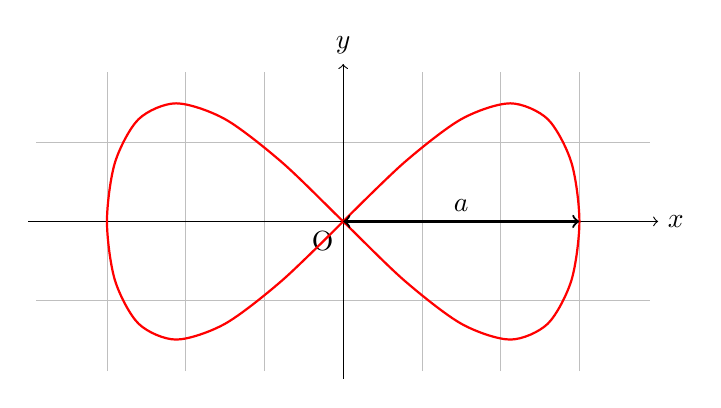
\begin{tikzpicture}
							\draw[gray,very thin, opacity = 0.5] (-3.9,-1.9) grid (3.9,1.9) [step=0.25cm];
							\draw[->] (-4,0) -- (4,0) node[right] {$x$};
							\draw[->] (0,-2) -- (0,2) node[above] {$y$};
							\draw[] (0,0) node[below left] {O};
	
							% draw figure 8 having a = 3
							\draw[thick, color = red ,variable=\t,domain=0.0:360, smooth]
								plot ({3 * sin(\t)},{3 * sin(\t) * cos(\t)});
							\draw[<->, thick] (0,0) -- node[above] {$a$} ++ (3,0) ;
						\end{tikzpicture}}
					\caption{Figure eight trajectory (where $a = 3$)}
					\end{figure}
			
				\item[$\blacktriangleright$]Curtate Cycloid, the path traced out by a fixed point at a radius $d<r$, where $r$ is the radius of a rolling circle. It is described by equations:
				\[x_{ref} = rt - d\sin(t) \qquad (\dot{x_{ref}} = r - d\cos(t) ) \]
				\[y_{ref} = d - d\cos(t) \qquad (\dot{y_{ref}} = d \sin(t)) \]
				Where $r$ is the radius of the rolling circle, and $d$ is the distance of the point drawing the 
				cycloid from the center such circle ($d<r$ to have a curtate cycloid).

				\begin{figure}[H]
					\makebox[\textwidth][c]{
						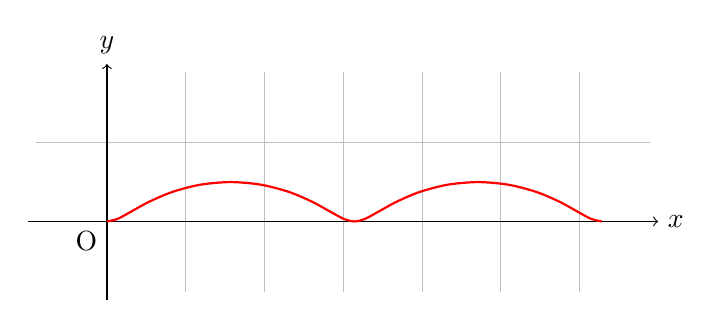
\begin{tikzpicture}
							\draw[gray,very thin, opacity = 0.5] (-0.9,-0.9) grid (6.9,1.9) [step=0.25cm];
							\draw[->] (-1,0) -- (7,0) node[right] {$x$};
							\draw[->] (0,-1) -- (0,2) node[above] {$y$};
							\draw[] (0,0) node[below left] {O};
	
							% draw cycloid having r = 0.5 and d = 0.25
							\draw[thick, color = red ,variable=\t,domain=0.0:4*pi, smooth]
								plot ({0.5 *\t - 0.25 * sin(deg(\t))},{0.25 -0.25 * cos(deg(\t))});
						\end{tikzpicture}}
					\caption{Cycloidal trajectory (where $r = 0.5$ and $d = 0.25$)}
					\end{figure}

		\end{itemize}
	\item[\textcolor{BlueGreen}{$\blacksquare$}] \textbf{Reference Transformation} which is in charge of performing a coordinate
		transformation from robot frame (attached to its center of gravity) to the P frame, where P is the point around which we
		are performing the feedback linearization of the bicycle model. \\
		Since the trajectory will be tracked by point P, and not by the COG of the robot, we have to apply a reference transformation
		to every trajectory setpoint in order to achieve the desired behaviour. \\
		The required transformation is:
			\[ x_{P_{ref}} = x_{ref} + \overrightarrow{PL} \cdot \cos(\theta) \]
			\[ y_{P_{ref}} = y_{ref} + \overrightarrow{PL} \cdot \sin(\theta) \]
		Where $x_{P_{ref}}$ and $y_{P_{ref}}$ are the setpoints for point P, $x_{ref}$ and $y_{ref}$ are the setpoints generated by
		the \textit{Trajectory Generator}, $\overrightarrow{PL}$ is the distance between point P and the COG of the robot, and $\theta$
		is the robot velocity direction (yaw of the robot).
	\item[\textcolor{BlueGreen}{$\blacksquare$}] \textbf{Output Transformation}, for the same reasons we introduced the \textit{Reference Transformation}
		we need an analogous transformation for the robot odometry data obtained through the "\textit{\textbackslash{}vesc\textbackslash{}odom}" topic:
		from the coordinates of the COG we need to retrieve the coordinates of point P which are the control variables of the \textit{Trajectory Tracker}. \\
		The required transformation is:
			\[ x_{P} = x + \overrightarrow{PL} \cdot \cos(\theta) \]
			\[ y_{P} = y + \overrightarrow{PL} \cdot \sin(\theta) \]
		Where $x_{P}$ and $y_{P}$ are the coordinates of point P, $x$ and $y$ are the coordinates of the robot COG, $\overrightarrow{PL}$ is the distance 
		between point P and the COG of the robot, and $\theta$ is the robot velocity direction (yaw of the robot).
	\item[\textcolor{BlueGreen}{$\blacksquare$}] \textbf{Trajectory Tracker} which is a controller in charge of performing trajectory tracking on 
		point P. \\
		Since we have two independent process variables $x_{P}$ and $y_{P}$, we have two independent PID (Proportional-Integral-Derivative) controllers to 
		achieve the trajectory tracking task. \\
		The \textit{Trajectory Generator} generates both position and velocity setpoints, thus we can use the latter as feed forward terms to increase the
		stability of the trajectory tracking controllers. \\
		The position errors are computed as:
		\[ x_{P_{err}} = x_{P_{ref}} - x_{P} \]
		\[ y_{P_{err}} = y_{P_{ref}} - y_{P} \]
		The control actions are:
		\[ v_{P_{x}} = \dot{x_{P_{ref}}} + K_p \cdot x_{P_{err}} + K_i \cdot x_{int} + K_d \cdot x_{der} \]
		\[ v_{P_{y}} = \dot{y_{P_{ref}}} + K_p \cdot y_{P_{err}} + K_i \cdot y_{int} + K_d \cdot y_{der} \]
		Where $\dot{x_{P_{ref}}}$ and $\dot{y_{P_{ref}}}$ are the feed forward terms, 
		$x_{int}$ and $y_{int}$ are the integrals of the variables, approximated using Riemann sums:
		\[ x_{int_t} = x_{int_{t-1}} + x_{P_{err}} \cdot \Delta t \]
		\[ y_{int_t} = y_{int_{t-1}} + y_{P_{err}} \cdot \Delta t \]
		
		Lastly, $x_{der}$ and $y_{der}$ are the derivatives of the errors, computed using finite differences:
		\[ x_{der} = \frac{x_{P_{err_t}} - x_{P_{err_{t-1}}}}{\Delta t} \]
		\[ y_{der} = \frac{y_{P_{err_t}} - y_{P_{err_{t-1}}}}{\Delta t} \]

		The PID controllers are identical for both process variables, here we present the schematic of the PID controlling $x_P$:
		\begin{figure}[H]
			\makebox[\textwidth][c]{
			\begin{tikzpicture}
				% nodes
				\node[circle, draw, fill=white] (sum1) {};

				\node[draw, fill=BlueGreen, minimum height=1cm, minimum width=1cm, right = 2cm of sum1] (i) {$\frac{K_i}{s}$};
				\node[draw, fill=BlueGreen, minimum height=1cm, minimum width=1cm, above = 0.5cm of i] (p) {$K_p$};
				\node[draw, fill=BlueGreen, minimum height=1cm, minimum width=1cm, below = 0.5cm of i] (d) {$sK_d$};

				\node[circle, draw, fill=white, right = 1cm of i] (sum2) {};
				\node[circle, draw, fill=white, right = of sum2] (sum3) {};
				
				% edges
				\draw[-{Triangle}] ($(sum1.west) + (-1, 0)$) -- ($(sum1.west)$)
					node[at start, left]{$x_{P_{ref}}$}
					node[near end, above]{$\scriptstyle+$};
				\draw[-{Triangle}] ($(sum1.south) + (0, -1)$) -- ($(sum1.south)$)
					node[at start, below]{$x_{P}$}
					node[near end, left]{$\scriptstyle-$};

				\draw[-{Triangle}] ($(sum1.east)$) -- ++(1cm,0) |- ($(p.west)$);
				\draw[-{Triangle}] ($(sum1.east)$) -- ++(1cm,0) -- ($(i.west)$);
				\draw[-{Triangle}] ($(sum1.east)$) -- ++(1cm,0) |- ($(d.west)$);

				\draw[-{Triangle}] ($(p.east)$) -- ++(1.2cm,0) -- ($(sum2.north)$)
					node[near end, left]{$\scriptstyle+$};
				\draw[-{Triangle}] ($(i.east)$) -- ($(sum2.west)$)
					node[near end, above]{$\scriptstyle+$};
				\draw[-{Triangle}] ($(d.east)$) -- ++(1.2cm,0) -- ($(sum2.south)$)
					node[very near end, left]{$\scriptstyle+$};

				\draw[-{Triangle}] ($(sum2.east)$) -- ($(sum3.west)$)
					node[near end, above]{$\scriptstyle+$};
				\draw[-{Triangle}] ($(sum3.north) + (0, 1)$) -- ($(sum3.north)$)
					node[at start, above]{$\dot{x_{P_{ref}}}$}
					node[near end, left]{$\scriptstyle+$};

				\draw[-{Triangle}] ($(sum3.east)$) -- ($(sum3.east) + (1,0)$)
					node[at end, right]{$v_{P_{x}}$};
			\end{tikzpicture}}
			\caption{PID schematic for controlling $x_P$}
		\end{figure}
\end{itemize}

\subsection{Configuration}
The node can be configured through the parameters present in the \\ \textit{trajectory\_tracker.yaml} configuration file, in particular we have:

\begin{center}
	\begin{xltabular}{\textwidth}{|>{\centering\arraybackslash \hsize=.25\hsize \linewidth=\hsize }X| 
							      >{\centering\arraybackslash \hsize=.15\hsize \linewidth=\hsize }X|
								  >{ \hsize=.6\hsize \linewidth=\hsize }X|}
	
		\hline
		\textbf{Parameter Name} &\textbf{Values Domain} &  \centering\arraybackslash \textbf{Description} \\
		\hline
		trajectory\_type & ${0,1,2,3,4}$ & Desired trajectory shape. \newline
		Values:
		\begin{itemize}
			\item[\textbf{0}] linear trajectory;
			\item[\textbf{1}] parabolic trajectory;
			\item[\textbf{2}] circular trajectory;
			\item[\textbf{3}] eight-shape trajectory;
			\item[\textbf{4}] cycloidal trajectory.
		\end{itemize} \\
		\hline
		\hline
		a\_coeff & $\mathbb{R}$ & 
		\multirow{2}{=}{The line describing the linear trajectory is parallel to the 
						direction vector: \[\vec{d}=(a\_coeff,b\_coeff) \]
						\newline (only used when \textit{trajectory\_type}=0)} \\
		& & \\
		& & \\
		\cline{1-2}
		b\_coeff & $\mathbb{R}$ & \\
		& & \\
		& & \\
		\hline
		\hline
		focal\_length & $\mathbb{R}$ & Focal length '$a$' [m] of the parabolic trajectory described by equation $y = ax^2$.
								\newline\newline(only used when \textit{trajectory\_type}=1) \\
		\hline
		\hline
		R & $\mathbb{R}^{+}$ & Radius of the circular trajectory [m]. \newline\newline(only used when \textit{trajectory\_type}=2)\\
		\hline
		W & $\mathbb{R}^{+}$ & Angular velocity of the circular trajectory [rad/s]. \newline\newline(only used when \textit{trajectory\_type}=2)\\
		\hline
		\hline
		a & $\mathbb{R}^{+}$ & Amplitude of the eight shape trajectory [m]. \newline\newline(only used when \textit{trajectory\_type}=3)\\
		\hline
		w & $\mathbb{R}^{+}$ & Angular velocity of the eight shape trajectory [rad/s]. \newline\newline(only used when \textit{trajectory\_type}=3)\\
		\hline
		\hline
		cycloid\_radius & $\mathbb{R}^{+}$ & Radius of the wheel [m]. \newline\newline(only used when \textit{trajectory\_type}=4)\\
		\hline
		cycloid\_distance & $\mathbb{R}^{+}$ & Distance from the center of the wheel to the point drawing the cycloid ($d<r$) [m]. \newline\newline(only used when \textit{trajectory\_type}=4)\\
		\hline
		\hline
		Kp &  $\mathbb{R}^{+}$ & Proportional gain for both PID controllers \\
		\hline
		Ki &  $\mathbb{R}^{+}$ & Integral gain for both PID controllers \\
		\hline
		Kd &  $\mathbb{R}^{+}$ & Derivative gain for both PID controllers \\
		\hline
		FFWD &  ${0,1}$ & Feedforward flag for both PID controllers. \newline
							Values: \begin{itemize}
								\item[\textbf{0}] disable feedforward component;
								\item[\textbf{1}] enable feedforward component;
							\end{itemize} \\
		\hline
		\hline
		PL\_distance &  $\mathbb{R}^{+}$ & Distance from the odometric centre of the robot to the selected point P used for the 
											linearization \\
		\hline
	\end{xltabular}
\end{center}

\subsection{Dynamic reconfigure}
The package uses \textit{dynamic reconfigure} to update some parameters at runtime without having to restart the node.
In particular, it can be used to change the PIDs configuration: $K_p$, $K_i$, $K_d$ and FFWD values. \\
Furthermore, the user can also toggle a boolean flag called "active" to start the trajectory generation (and tracking)
process at will.

\subsection{Choiche of PID controller and parameters}

Performing an empiric PID tuning, we achieved good performances with a P controller with feed forward enabled; thus setting:
\[ K_p = 5 \qquad K_i = 0  \]
\[ K_d = 0 \qquad FFWD = true \]